\documentclass[11pt]{article}

% "preprint": non-anonymous, with page numbers (course progress report).
\usepackage[preprint]{acl}

\usepackage{times}
\usepackage{latexsym}
\usepackage[T1]{fontenc}
\usepackage[utf8]{inputenc}
\usepackage{microtype}
% \usepackage{inconsolata}  % optional in the ACL template; not installed here
\usepackage{graphicx}
\usepackage{booktabs}
\usepackage{amsmath}
\usepackage{multirow}

\newcommand{\matra}{m\=atr\=a}
\newcommand{\Matra}{M\=atr\=a}
\newcommand{\tala}{t\=ala}
\newcommand{\Tala}{T\=ala}
\newcommand{\avartan}{\=avartan}
\newcommand{\vibhag}{vibh\=ag}
\newcommand{\Vibhag}{Vibh\=ag}
\newcommand{\Avartan}{\=Avartan}
\newcommand{\khali}{kh\=al\={\i}}
\newcommand{\tihai}{tih\=a\={\i}}
\newcommand{\Tihai}{Tih\=a\={\i}}
\newcommand{\tintal}{t\={\i}nt\=al}
\newcommand{\kayda}{k\=ayd\=a}
\newcommand{\gharana}{ghar\=an\=a}

\title{Learning an Interpretable Probabilistic Grammar of Hindustani \Tala:\\ Mid-Semester Progress Report}

\author{Rishav Kumar Gupta \\
  ID: 2023A7PS0526P \\
  BITS Pilani, Pilani Campus \\
  \texttt{f20230526@pilani.bits-pilani.ac.in} \\
  Under the guidance of Prof.\ Yash Sinha}

\begin{document}
\maketitle

\begin{abstract}
We are building a probabilistic grammar of tabla rhythm in t\={\i}nt\=al whose
derivation trees are themselves the explanation of each generated or analysed
composition. This report covers the work completed so far on the 38-composition
Mulgaonkar Tabla Solo corpus: a verified data pipeline, a timing-grounded
representation, a supervised PCFG, an Inside--Outside EM study, an attribute
layer that enforces cycle length and the \tihai{} landing constraint, a
held-out study of parameter tying, and a generator that outputs a sequence,
its derivation tree and its rule history together. Main findings: (i)~the
context-free grammar alone never produces a valid 16-\matra{} cycle (0/2000
samples), and the attribute layer that fixes this also lowers held-out cost by
0.77 bits per stroke (about 15\%); (ii)~even EM started at the correct
supervised probabilities drifts away from them, because parsing untimed bol
strings is highly ambiguous; (iii)~of 115 symbolic \tihai{} candidates, only
5 also satisfy the metrical constraint (at a 0.15-\matra{} tolerance); (iv)~sam is the only metrical position
whose statistics measurably differ, and the \khali{} \vibhag{} shows no
detectable effect; and (v)~generated material repeats 4-stroke patterns far
less than real compositions (median 3\% vs.\ 68\%). Baseline comparisons and
human evaluation remain to be done.
\end{abstract}

\section{Introduction}

Hindustani rhythm is organised by \tala{}, a cycle (\avartan{}) of beats
(\matra{}) grouped into sections (\vibhag{}); t\={\i}nt\=al has 16 \matra{} in four
\vibhag{}s of four, with the cycle resolving on its first beat, sam, and its
third \vibhag{} marked as \khali{} \citep{clayton2000time}. Tabla
compositions are written and recited as sequences of stroke syllables (bols),
and are built from named, hierarchical operations: theme and variation in a
\kayda{}, and the \tihai{}, a phrase played three times so that it ends on
sam.

This structure invites a grammatical treatment. Grammars of tabla already
exist: the Bol Processor encoded tabla idioms as formal grammars elicited from
expert musicians \citep{kippen1989identification,kippen1992modelling}. Our aim
differs in two ways. The production \emph{probabilities} are learned from a
corpus rather than elicited, and the grammar is compared quantitatively
against black-box sequence models. The motivation is interpretability in the
sense of \citet{rudin2019stop}: a generated composition should come with its
derivation tree, an explanation that is the model's own production history,
not a post-hoc account.

The project asks four questions. RQ1: does a corpus-fit grammar predict
held-out compositions as well as matched-capacity black-box models? RQ2: do
its high-probability rules correspond to recognised tabla units? RQ3: do
derivation trees help people on rhythm tasks? RQ4: what formal power does
\tala{} structure require? This report covers the groundwork for all four and
the first answers to RQ4. Contributions so far:

\begin{itemize}
\setlength\itemsep{0pt}
\item A verified, reproducible pipeline for the corpus, with a representation
  that places every stroke in the metrical grid using its onset time (\S\ref{sec:data}).
\item A supervised PCFG, a CYK/Inside parser and an Inside--Outside EM study
  showing that the untimed parsing problem is highly ambiguous (\S\ref{sec:pcfg}).
\item An attribute layer \citep{knuth1968semantics} that enforces cycle length
  and checks the \tihai{} arithmetic against real timing, and a constrained
  generator (\S\ref{sec:attr}).
\item A held-out study of which metrical positions need their own parameters
  (\S\ref{sec:tying}), and an analysis of what the generator does and does
  not reproduce (\S\ref{sec:gen}).
\end{itemize}

\section{Related Work}

\paragraph{Grammars of tabla.} The Bol Processor project modelled tabla
improvisation with formal grammars and used them in fieldwork with expert
musicians \citep{kippen1992modelling}, and studied grammatical inference from
expert-approved examples \citep{kippen1989identification}. It is the direct
precedent for this work; our delta is corpus-estimated probabilities,
attribute constraints, and quantitative comparison with sequence models.

\paragraph{Probabilistic grammars of music.} Generative syntax has been
developed for tonal and jazz harmony \citep{rohrmeier2011towards}, combined
with a grammar of rhythm and metre, which improved the harmonic model
\citep{harasim2019harmonic}, and supported by a treebank of hierarchical
analyses \citep{harasim2020jazz}. Minimum-description-length methods have been
used to choose among musical structure models \citep{mavromatis2009minimum}.
Probabilities of context-free grammars are classically estimated with the
Inside--Outside algorithm \citep{lari1990estimation}.

\paragraph{Computational analysis of Indian rhythm.} Data-driven metre
analysis of Indian art music is developed in \citet{srinivasamurthy2016data}.
Our corpus comes from \citet{gupta2015discovery}, who discovered syllabic
percussion patterns in tabla solo recordings.

\section{Data and Representation}
\label{sec:data}

\paragraph{Corpus.} The Mulgaonkar Tabla Solo dataset \citep{gupta2015discovery}
has 38 t\={\i}nt\=al compositions from six \gharana{}s (Punjab 11, Benaras 9, Dilli
6, Ajrada 5, Lucknow 4, Farukkhabad 3) and 20 composition types. Each comes
with a score and two time-aligned onset files: one in a raw 40-symbol bol
vocabulary, and one mapped by the dataset authors to 18 symbols. We
verified that every score matches its raw onset sequence exactly, token by
token (38/38). Compositions range from 47 to 611 onsets (mean 217.0).
Rests (`\texttt{-}', 1{,}117 occurrences) appear only in the scores; the onset
files have no rests and no durations. We use the 18-symbol vocabulary
throughout, because many raw symbols are rare spelling variants of one stroke.
The annotations are licensed CC BY-NC-ND 4.0; the audio is not redistributed.

\paragraph{Splits.} Composition-level train/validation/test splits of 26/6/6
(seed 42). The two versions of one composition (\texttt{ajr\_10\_ajr},
\texttt{ajr\_10\_dli}) are kept in the same split to prevent leakage. The
test split has not been used in any analysis reported here.

\paragraph{Representation.} The hierarchy is
Composition~$\to$~\Avartan~$\to$~\Vibhag~$\to$~\Matra~$\to$~stroke.
\Avartan{} boundaries come from score lines. The score notation does not
reliably say which \matra{} each token belongs to (group sizes vary with the
subdivision), so instead each \avartan{} is divided into 16 equal \matra{}s
and every stroke is placed by its onset time. This yields 351 \avartan{}s
and 8{,}245 strokes, with no onset lost. The equal-\matra{} assumption is
approximate: positions within a \matra{} are imprecise (\S\ref{sec:attr}).

\section{A Supervised PCFG and the Cost of Ambiguity}
\label{sec:pcfg}

\paragraph{Grammar.} Every non-terminal encodes a structural fact checked in
earlier stages: \texttt{Composition} is a list of \texttt{Avartan}s; an
\texttt{Avartan} is four \texttt{Vibhag}$_i$; a \texttt{Vibhag} is four
\matra{}s, the first of the cycle being \texttt{SamMatra}; and a \matra{} is a
list of \texttt{BolSlot}s, each emitting one bol. Because each \avartan{}'s
derivation is known from timing, probabilities are estimated by supervised
maximum likelihood: 9 non-terminals, 44 rules (18 terminal). The named
\kayda{} categories (mukh, pal\d{t}\=a, etc.) are not used yet: the
corpus has no annotations from which they could be assigned reliably.

\paragraph{Parsing untimed strings is highly ambiguous.} We implemented a
CYK/Inside algorithm that sums over all parses. On three compositions its
total log-probability far exceeds that of the single known derivation
(Table~\ref{tab:ambig}). Without timing, the same bol string can be split into
\matra{}s and \vibhag{}s in a very large number of grammatical ways. CYK
runtime grew from 0.16\,s ($n{=}47$) to 1.50\,s ($n{=}96$) and 57.65\,s
($n{=}256$), steeper than cubic. Real recordings therefore have to be scored
with their timing-derived derivation, not by parsing.

\begin{table}[t]
\centering\small
\begin{tabular}{lrrrr}
\toprule
Comp. & $n$ & Known tree & Inside & $\Delta$ \\
\midrule
pjb\_84 & 47 & $-184.45$ & $-120.60$ & $+63.86$ \\
ajr\_12 & 96 & $-363.23$ & $-252.52$ & $+110.71$ \\
luc\_17 & 164 & $-530.64$ & $-348.96$ & $+181.68$ \\
\bottomrule
\end{tabular}
\caption{Log-probability (nats) of the known timing-derived derivation vs.\
the Inside total over all parses of the same untimed bol string.}
\label{tab:ambig}
\end{table}

\paragraph{Inside--Outside EM.} The project plan prescribes EM, initialised
from supervised estimates ``to avoid poor local optima''. We tested this
claim by running EM on all 351 \avartan{}s from three initialisations (20
iterations, Dirichlet $\alpha{=}0.01$; Table~\ref{tab:em}). The predicted
ranking held at every iteration, but the final gaps were small (about 0.1\%).
More importantly, \emph{EM started at the supervised probabilities moved away
from them}: for example, $P(\texttt{Avartan}\to\texttt{Vibhag}_2\,\texttt{Vibhag}_3)$
went from 0.32 to 0.46. EM maximises the probability of the untimed string,
which is dominated by spurious segmentations, so it is not a safe refinement
here. We keep the supervised grammar.

\begin{table}[t]
\centering\small
\begin{tabular}{lrr}
\toprule
Initialisation & Iteration 1 & Iteration 20 \\
\midrule
Supervised & $-19037.83$ & $\mathbf{-19000.33}$ \\
Uniform & $-25597.38$ & $-19009.39$ \\
Random (Dirichlet(1)) & $-35406.80$ & $-19017.56$ \\
\bottomrule
\end{tabular}
\caption{Corpus log-likelihood (nats, 351 \avartan{}s) under Inside--Outside EM.}
\label{tab:em}
\end{table}

\section{Attribute Layer and the \Tihai{} Constraint}
\label{sec:attr}

\paragraph{The grammar cannot count.} Its list rules reuse a label
(\texttt{Avartan}~$\to$~\texttt{Vibhag}$_0$~\texttt{Avartan}), so nothing
tracks how many \matra{}s have been placed: 0 of 2{,}000 free samples were a
valid cycle. Following attribute grammars \citep{knuth1968semantics}, every
node carries a start position (inherited) and a duration (synthesised), in
\matra{}s. Generation propagates the cycle constraint down the derivation:
only learned productions consistent with ``vibh\=ags and \matra{}s still to
place'' are allowed, with their probabilities renormalised. This gives
2{,}000/2{,}000 valid cycles. For t\={\i}nt\=al the constraint fixes the whole
skeleton; all remaining freedom lies inside the \matra{}s.

\paragraph{Empty \matra{}s.} Only 117/351 real \avartan{}s have a stroke in
every \matra{}, and 893 of 5{,}616 \matra{}s (15.9\%) are empty. Our first
grammar dropped them, losing the cycle length. Adding an explicit rest, using
the score's own `\texttt{-}', makes all 351 real cycles well-formed. It also
showed that the grammar's ``irregular'' cycle rules came entirely from silent
\vibhag{}s: with rests, \texttt{Avartan} has exactly three rules, each used 351
times. The rest symbol cannot tell silence from a sustained stroke.

\paragraph{Timing precision.} Within a \matra{}, only 17.5\% of strokes fall
within $\pm0.05$ of the beat (10\% by chance), 10.8\% near the half-\matra{}
(10\% by chance), and quarter positions are below chance. Whole-\matra{}
placement is reliable; fractional positions are approximate. We therefore
report real-data results at several tolerances.

\paragraph{The \tihai{} formula is ambiguous as written.} The planned
constraint $3\,d(p)+2\,d(g)+1 \equiv \textit{target} \pmod{16}$ does not say
what \textit{target} is measured from or what the ``$+1$'' is. We tested two
readings on real timing: (A) the last stroke of the third phrase is on sam;
(B) the stroke after it is. Table~\ref{tab:tihai} applies both to the 115
symbolic candidates (a phrase repeated three times with equal gaps). These
came from an exact-repetition search over all 38 compositions.

\begin{table}[t]
\centering\small
\begin{tabular}{crrrr}
\toprule
Tol. & A & B & Regular & Strict (B+reg.) \\
\midrule
0.10 & 8 & 17 & 53 & 4 \\
0.15 & 8 & 18 & 65 & 5 \\
0.25 & 9 & 19 & 87 & 12 \\
\bottomrule
\end{tabular}
\caption{Real \tihai{} candidates ($N{=}115$) satisfying each condition at a
given tolerance (\matra{}s). ``Regular'' means equal spacing between
phrases. By chance, about 5 would land under B (4.3\% of all onsets lie
within 0.15 of sam).}
\label{tab:tihai}
\end{table}

Reading B lands at about $3.6\times$ chance, reading A at about $1.6\times$, so
we adopt B. Only 5 candidates satisfy the full constraint at 0.15
\matra{}. Three of those come from one long repeating passage
(\texttt{luc\_18}) that is probably not a single \tihai{}. The clearest match
is in \texttt{ben\_25} (phrase $\approx$\,4.01 \matra{}, gap $\approx$\,0.95,
next stroke 0.000 \matra{} from sam; Figure~\ref{fig:tihai}). 55 candidates
have no gap, which the plan's allowed gaps $\{\tfrac14,\tfrac12,\tfrac34,1,
1\tfrac12,2\}$ exclude, and 25 of the 60 gapped ones fall outside that set.
None of this has yet been checked by a tabla expert.

\paragraph{Generating \tihai{}s.} A \tihai{} cycle is generated by sampling a
phrase of whole \matra{}s once, copying it three times, and placing it so the
stroke after it falls exactly on the next sam. The three-fold copy is a
dependency a context-free grammar cannot express for phrases of unbounded
length. All 200 generated compositions pass the same checker used on real
data. The symbol-only repetition search used to find real candidates
recovers the exact boundaries in only 94/200. In 93 more it finds the same pattern shifted by one token, because a
rest before the \tihai{} matches a rest gap on symbols alone; only durations
separate the two. Without the attribute layer, 300 generated sequences
contained no \tihai{} that landed on sam.

\begin{figure*}[t]
\centering
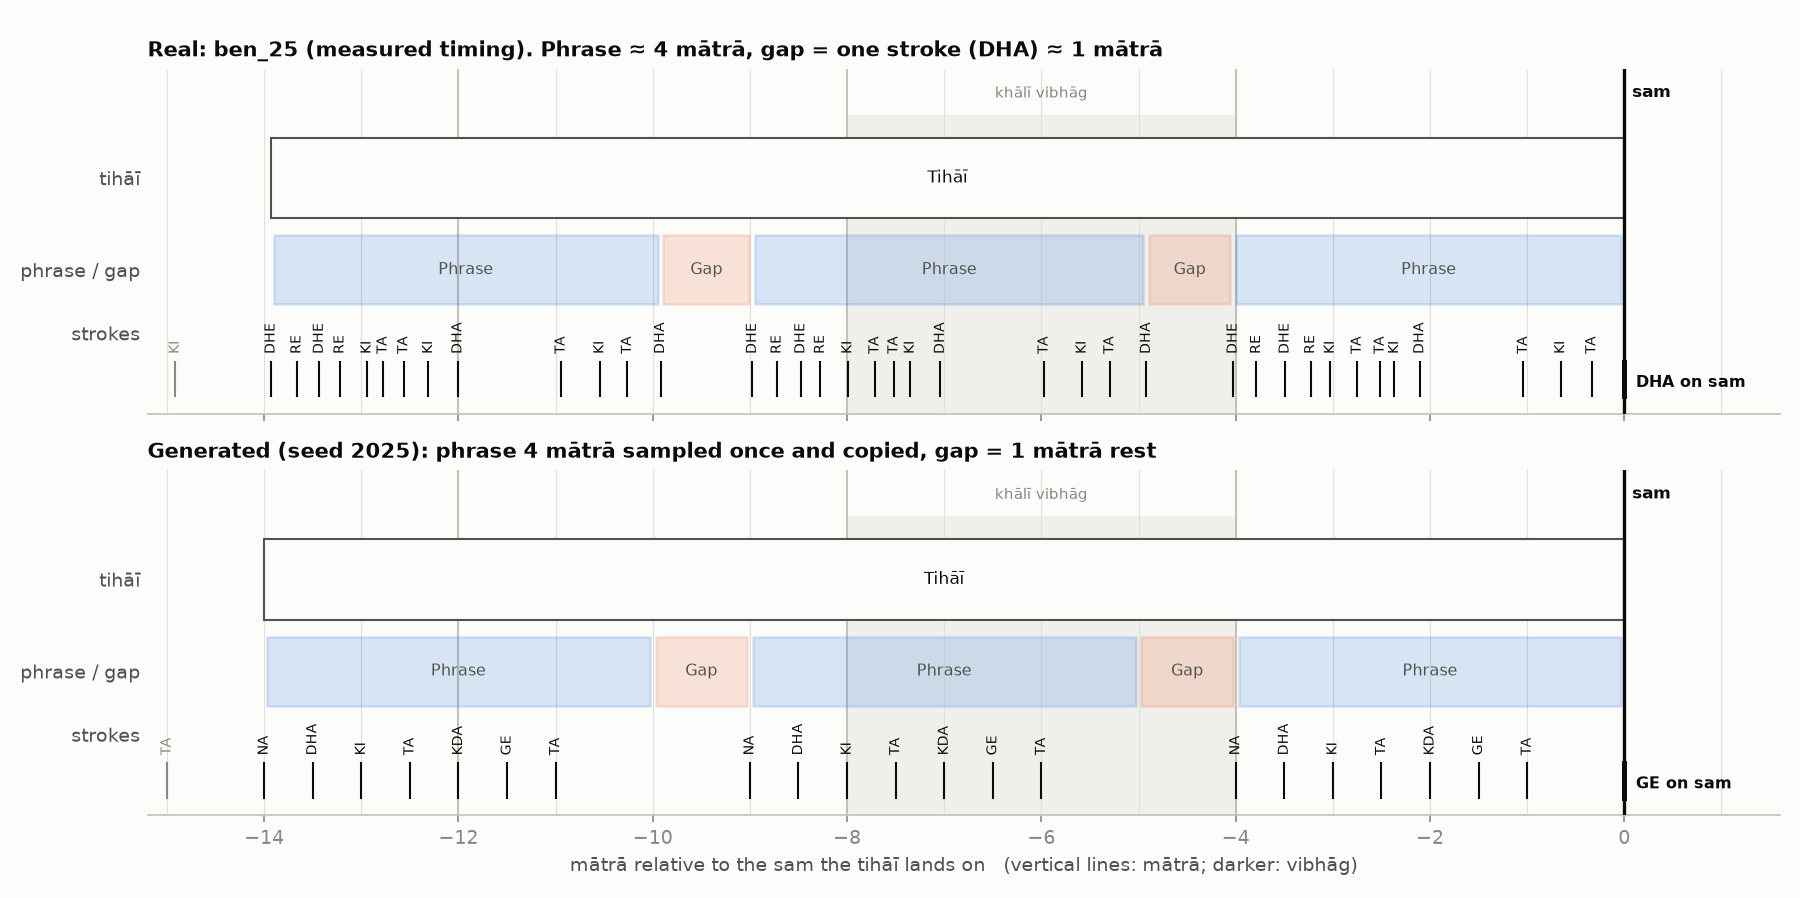
\includegraphics[width=0.92\textwidth]{figures/phase9_tihai_real_vs_generated.png}
\caption{A \tihai{} as a derivation laid out in time. Rows are tree levels
(\tihai{}, phrase/gap, strokes); every box spans the time its node covers,
counted in \matra{}s back from the sam where the \tihai{} lands. Top: real
(\texttt{ben\_25}, measured timing). Bottom: generated, with the same shape
(4-\matra{} phrase, 1-\matra{} gap).}
\label{fig:tihai}
\end{figure*}

\section{Which Positions Need Their Own Parameters?}
\label{sec:tying}

With the skeleton fixed by the attribute layer, the free parameters are two
tables. One gives the probability of each \emph{stroke}; the other gives the
\emph{shape} of a \matra{} (empty, one stroke, or more). Each table can be
shared across the cycle or split by sam, \khali{}, or \vibhag{}. We score each
variant by leave-one-out on the train and validation compositions only (31
units, 7{,}351 strokes, 319 cycles). We report held-out bits per stroke,
with paired bootstrap 95\% intervals over compositions.

\paragraph{The attribute layer improves prediction.} The plain CFG spends
exactly 17.774 bits per cycle describing a structure that never varies. Removing
that cost lowers held-out cost from 5.310 to 4.539 bits per stroke. Giving the
stroke list inside a \matra{} its own label (so ``is it empty'' and ``does the
list continue'' stop sharing probabilities) saves a further 0.127
$[0.076, 0.169]$ bits per stroke.

\begin{table}[t]
\centering\small
\setlength{\tabcolsep}{3pt}
\begin{tabular}{lrrc}
\toprule
Split (vs.\ base) & Par. & $\Delta$ & 95\% CI \\
\midrule
strokes by sam & 41 & $-0.0088$ & $[-0.0162, -0.0005]$ \\
strokes by \khali{} & 41 & $-0.0005$ & $[-0.0046, +0.0041]$ \\
strokes by \vibhag{} & 75 & $-0.0024$ & $[-0.0169, +0.0113]$ \\
shapes: merge sam & 21 & $+0.0117$ & $[+0.0059, +0.0175]$ \\
shapes: add \khali{} & 27 & $-0.0007$ & $[-0.0031, +0.0013]$ \\
\bottomrule
\end{tabular}
\caption{Held-out effect of tying choices, in bits per stroke (negative =
better). Base: one stroke table, shape table split by sam (24 parameters,
4.539 bits/stroke).}
\label{tab:tying}
\end{table}

\paragraph{Only sam differs.} Table~\ref{tab:tying} and
Figure~\ref{fig:grid} show that sam is the only position with measurable
effects. Merging sam's \matra{} shapes into the shared table hurts, and giving
sam its own stroke table helps a little (DHA is $2.25\times$ more frequent on
sam than overall). The \khali{} \vibhag{}, which tabla theory expects to differ, shows no
detectable effect in strokes or shapes. We can't yet say why: these are solo
compositions rather than the basic cycle pattern (\d{t}hek\=a), \vibhag{}
boundaries come from the equal-\matra{} assumption, and the bass and treble
parts of compound strokes have not been separated. Partial (soft) tying gave
no gain over a full split. All tying effects are at most about 0.3\% of the
total, against 15\% for the attribute layer. Before opening the test split we fixed
the grammar for the RQ1 comparison: rests, tail labels, and sam-specific
stroke and shape tables (41 parameters, 4.530 bits/stroke). This is the
simplest variant whose gain over the base excludes zero.

\begin{figure}[t]
\centering
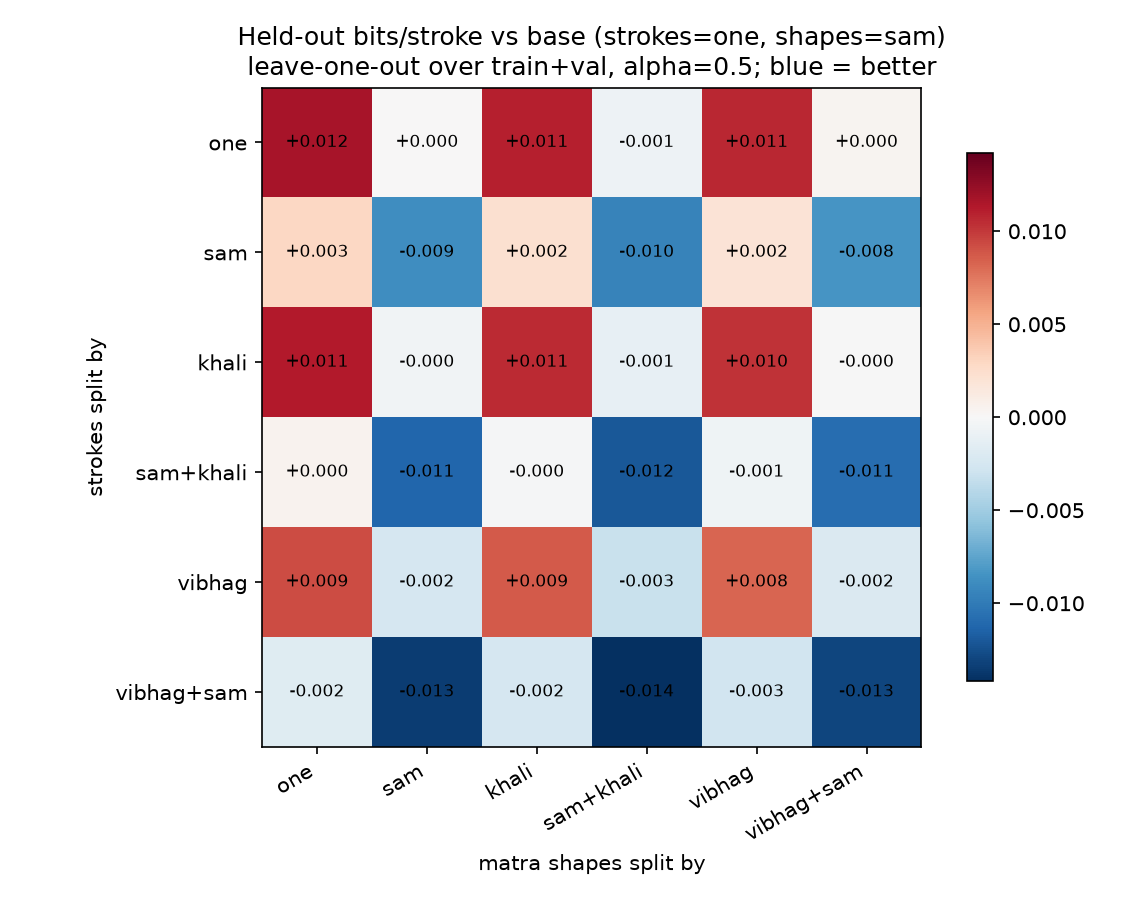
\includegraphics[width=\columnwidth]{figures/phase8_tying_grid.png}
\caption{Held-out bits/stroke relative to the base for all 36 combinations
of stroke tying (rows) and \matra{}-shape tying (columns). Blue is better.
Every improvement involves a sam split.}
\label{fig:grid}
\end{figure}

\section{Generation and What It Misses}
\label{sec:gen}

The selected grammar, trained on train and validation data (13 non-terminals,
58 rules), generates compositions as a timeline together with an annotated
derivation tree and its rule sequence; 20/20 seeded examples pass every
check. Figure~\ref{fig:stats} and Table~\ref{tab:gen} compare 400 generated
3-cycle stretches with the real data. The generator reproduces the quantities
it models: how many strokes fall in a \matra{}, and which strokes fall on sam.
Since it was trained on this data, that only checks the sampler. It fails on
repetition: in real compositions a 3-cycle window reuses a median 68\% of its
4-stroke patterns, against 3\% in generated ones. The grammar chooses each stroke from
its position alone, so its only repetition is the \tihai{} copy.

\begin{table}[t]
\centering\small
\begin{tabular}{lrr}
\toprule
 & Real & Generated \\
\midrule
Empty \matra{}s & 0.170 & 0.167 \\
\Matra{}s with 1 stroke & 0.391 & 0.397 \\
\Matra{}s with 2 strokes & 0.330 & 0.316 \\
DHA share on sam & 0.162 & 0.160 \\
4-gram repetition (median) & \textbf{0.680} & \textbf{0.034} \\
\bottomrule
\end{tabular}
\caption{Generated vs.\ real (train and validation) statistics.}
\label{tab:gen}
\end{table}

\begin{figure*}[t]
\centering
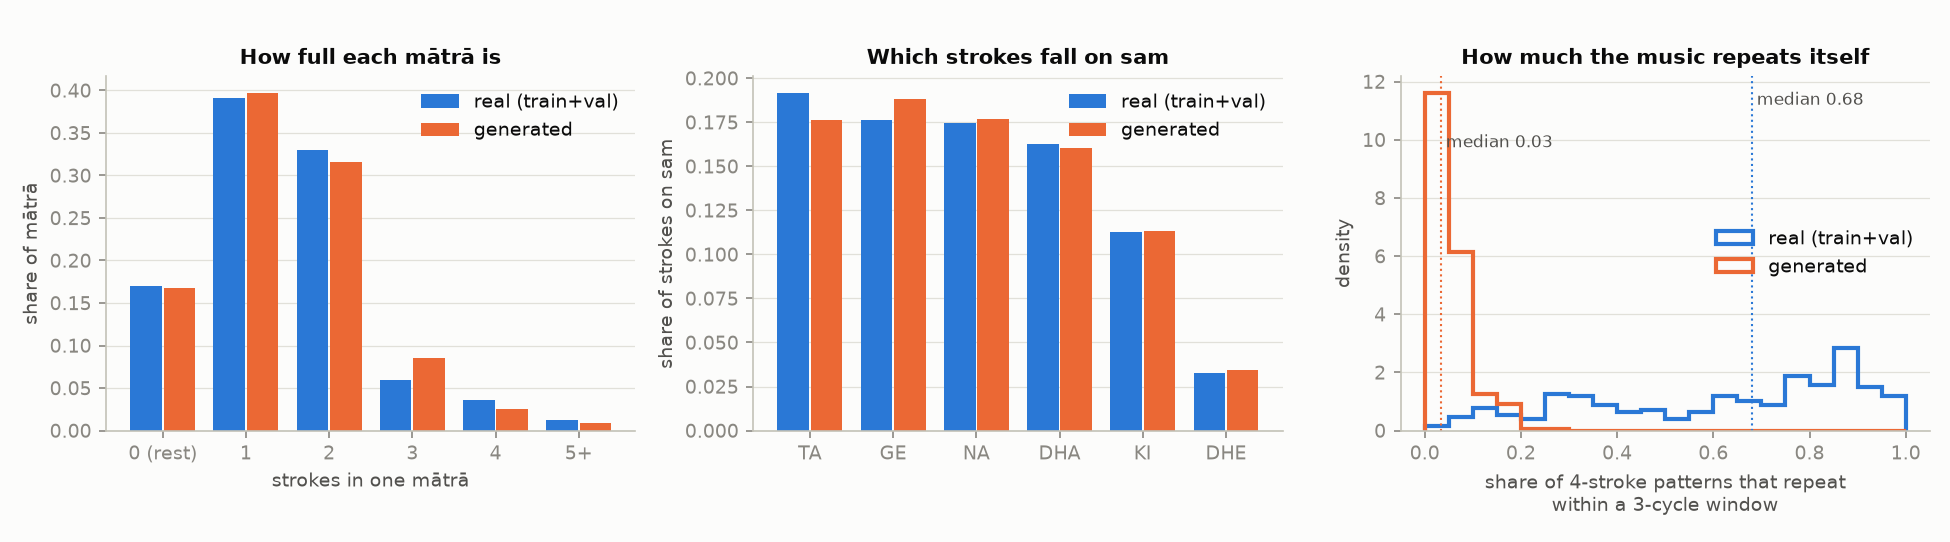
\includegraphics[width=0.95\textwidth]{figures/phase9_generated_vs_real_stats.png}
\caption{Generated (orange) vs.\ real (blue). Left and middle: quantities the
grammar models. Right: share of 4-stroke patterns that recur within a 3-cycle
window. Real tabla is strongly self-repetitive; the generator is not.}
\label{fig:stats}
\end{figure*}

\section{Next Steps}

\begin{itemize}
\setlength\itemsep{0pt}
\item \textbf{Baselines and RQ1.} Train bol $n$-gram, LSTM and Transformer
  models with documented capacity, and compare them with the fixed grammar on
  the untouched test split. First, decide how the baselines are scored: the
  grammar's cost covers strokes \emph{and} their placement, whereas a bol
  sequence model predicts strokes only. Given \S\ref{sec:gen}, we expect the
  current grammar to predict worse than the baselines; this is a hypothesis to
  test, not a result.
\item \textbf{Repetition.} Add productions that reuse and vary earlier
  phrases, which is what the \kayda{} vocabulary (mukh, dohr\=a, pal\d{t}\=a)
  describes, and measure the gain against the current grammar.
\item \textbf{Validation.} Expert review of the \tihai{} matches and of
  generated output; a small seed treebank; and the planned behavioural study
  (RQ3).
\end{itemize}

\section{Conclusion}

A corpus-trained tabla grammar becomes usable only once duration constraints
are enforced on top of it. Those constraints make every generated cycle
valid, check \tihai{} arithmetic against real timing, and also improve
held-out prediction. EM on untimed strings is unreliable because parsing them
is highly ambiguous. Of the metrical positions, only sam measurably changes
the statistics. The clearest gap is that real compositions repeat material
and the grammar does not, which is the next modelling target.

\section*{Limitations}

All results come from one corpus of 38 compositions by a single performer,
in one \tala{}, using the dataset's 18-symbol vocabulary; the 40-symbol
vocabulary has not been evaluated. Metrical positions rely on an
equal-\matra{} assumption whose sub-\matra{} precision is weak, so fractional
results are reported at several tolerances. No musicological judgement here
has been validated by a tabla expert, and the named \kayda{} categories are
not yet modelled. The \tihai{} formula required an interpretive choice
(reading B), made on corpus evidence. No baseline comparison or human
evaluation has been run yet; claims about RQ1--RQ3 are therefore deferred.
The implementation is checked by 65 regression tests, several of which caught
real errors during development before any results were reported.

\section*{Acknowledgments}

This work is carried out under the guidance of Prof.\ Yash Sinha at BITS
Pilani, Pilani Campus. We thank the creators of the Mulgaonkar Tabla Solo
dataset for making the scores and onset annotations available.

\bibliography{references}

\end{document}
